\section{Effect of Equity on Feedback Loop}
\begin{figure*}[h]
\centering
\begin{subfigure}[b]{0.33\textwidth}
\caption{$\beta=0.1$}
    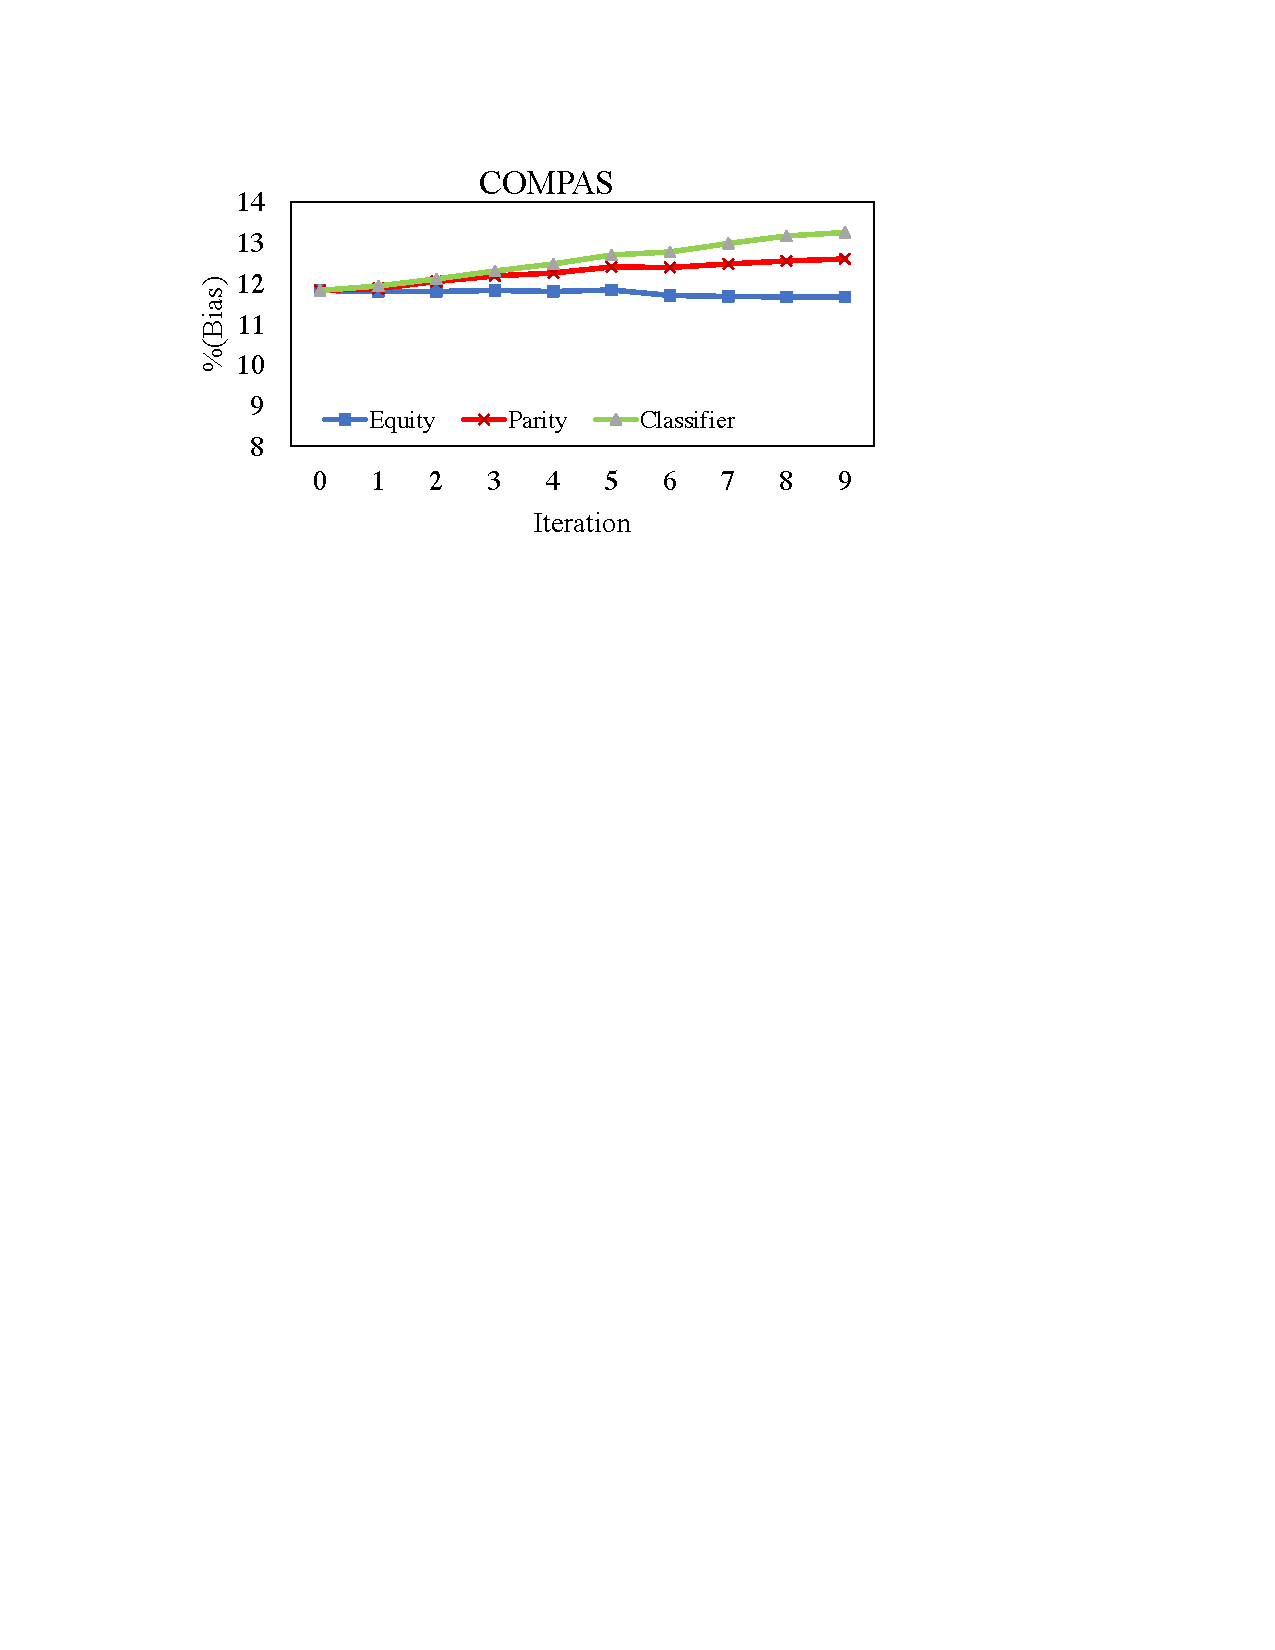
\includegraphics[width=\textwidth,trim=2.7cm 18cm 6.5cm 2.8cm,clip=true]{images/compas_per_01.pdf}
    \end{subfigure}
    \begin{subfigure}[b]{0.33\textwidth}
\caption{$\beta=0.5$}
     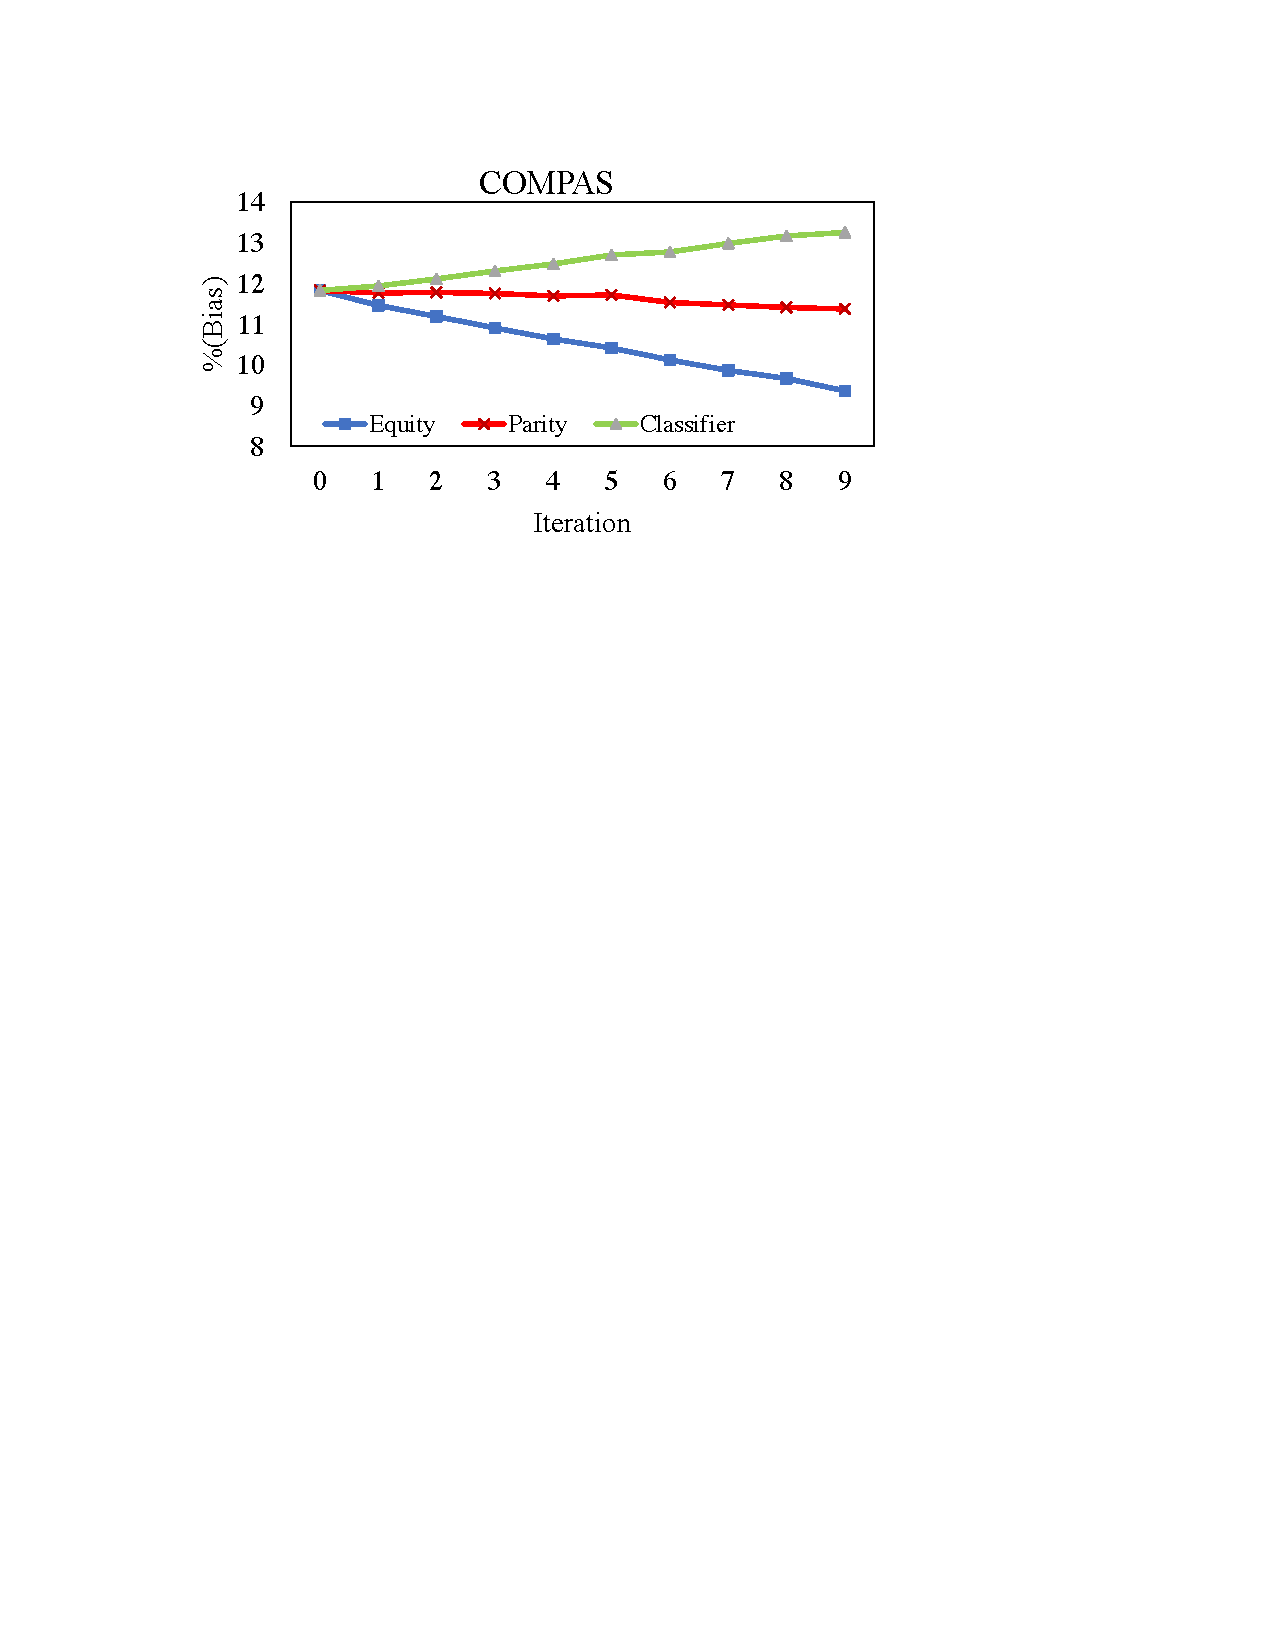
\includegraphics[width=\textwidth,trim=2.7cm 18cm 6.5cm 2.8cm,clip=true]{images/compas_per_05.pdf}
      \end{subfigure}
     \begin{subfigure}[b]{0.33\textwidth}
\caption{$\beta=0.9$}
      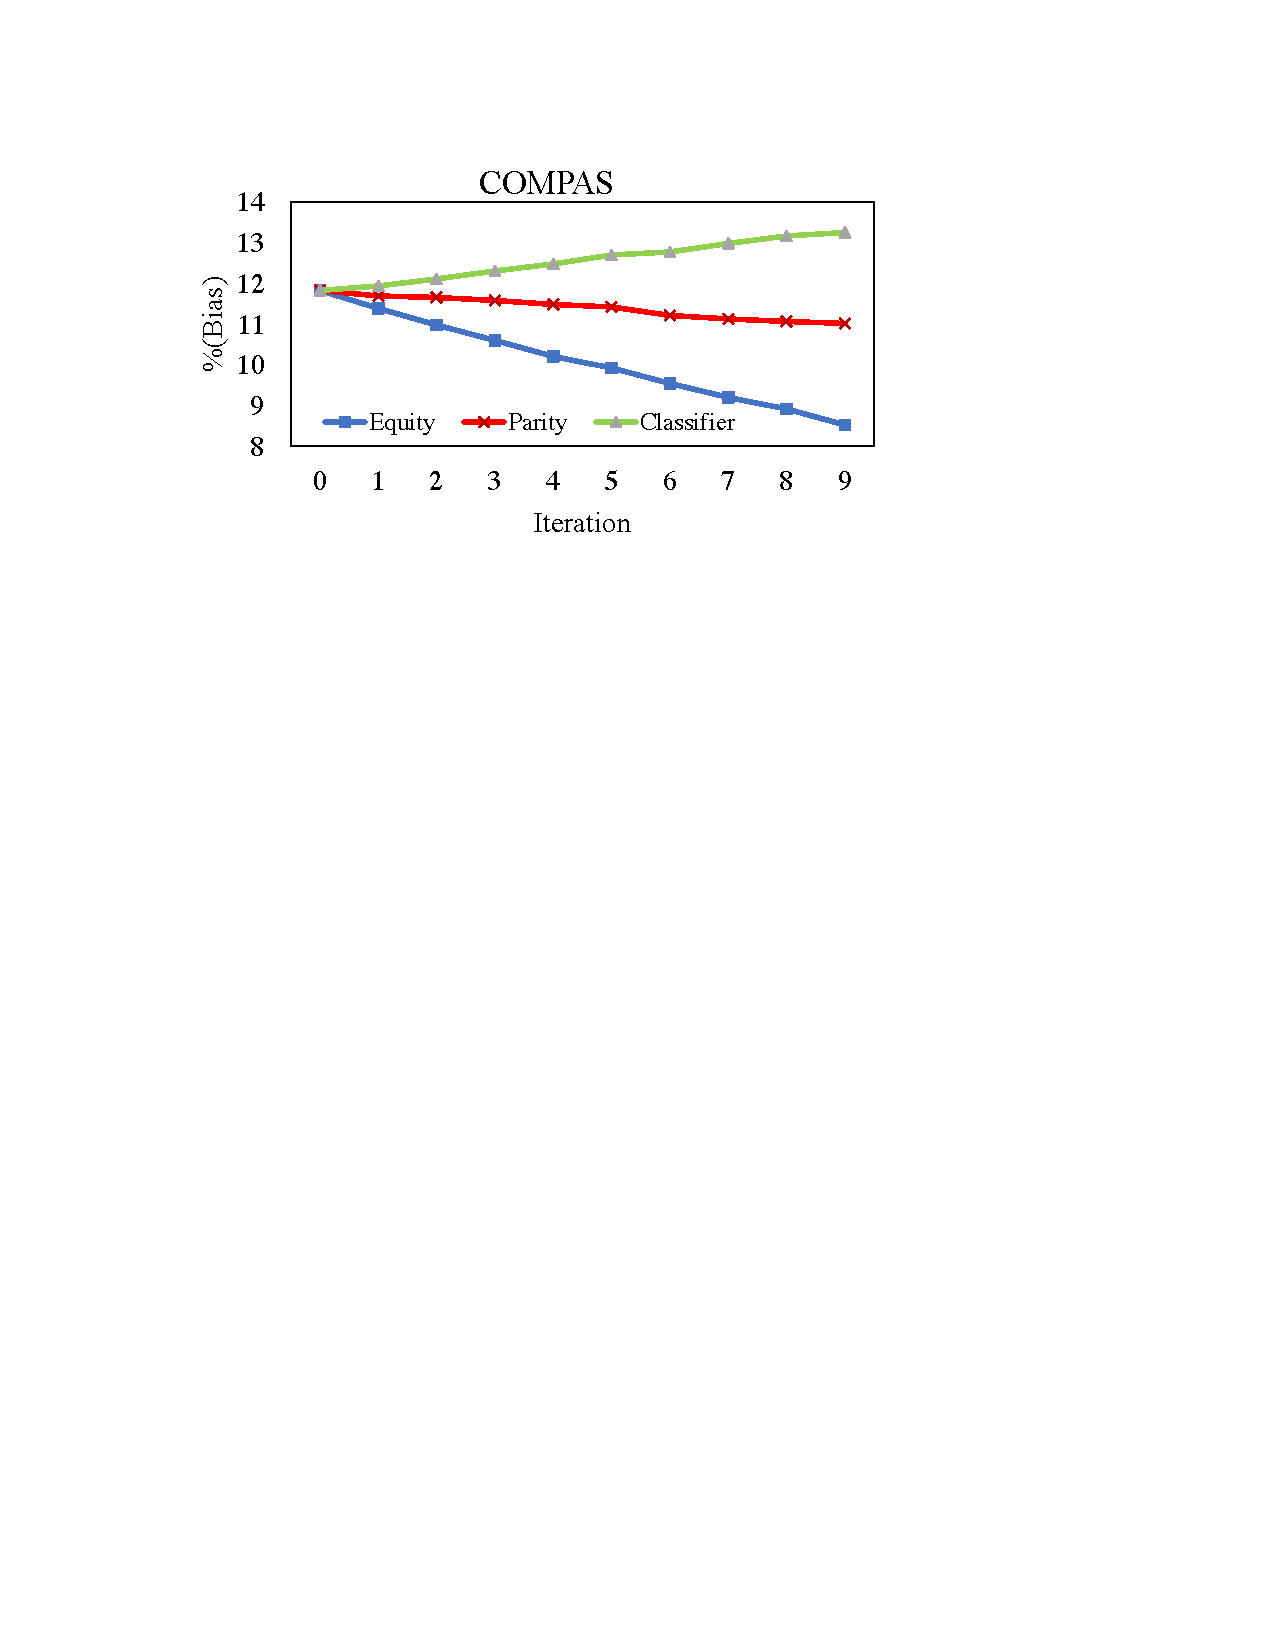
\includegraphics[width=\textwidth,trim=2.7cm 18cm 6.5cm 2.8cm,clip=true]{images/compas_per_09.pdf}
      \end{subfigure}
      \begin{subfigure}[b]{0.33\textwidth}
      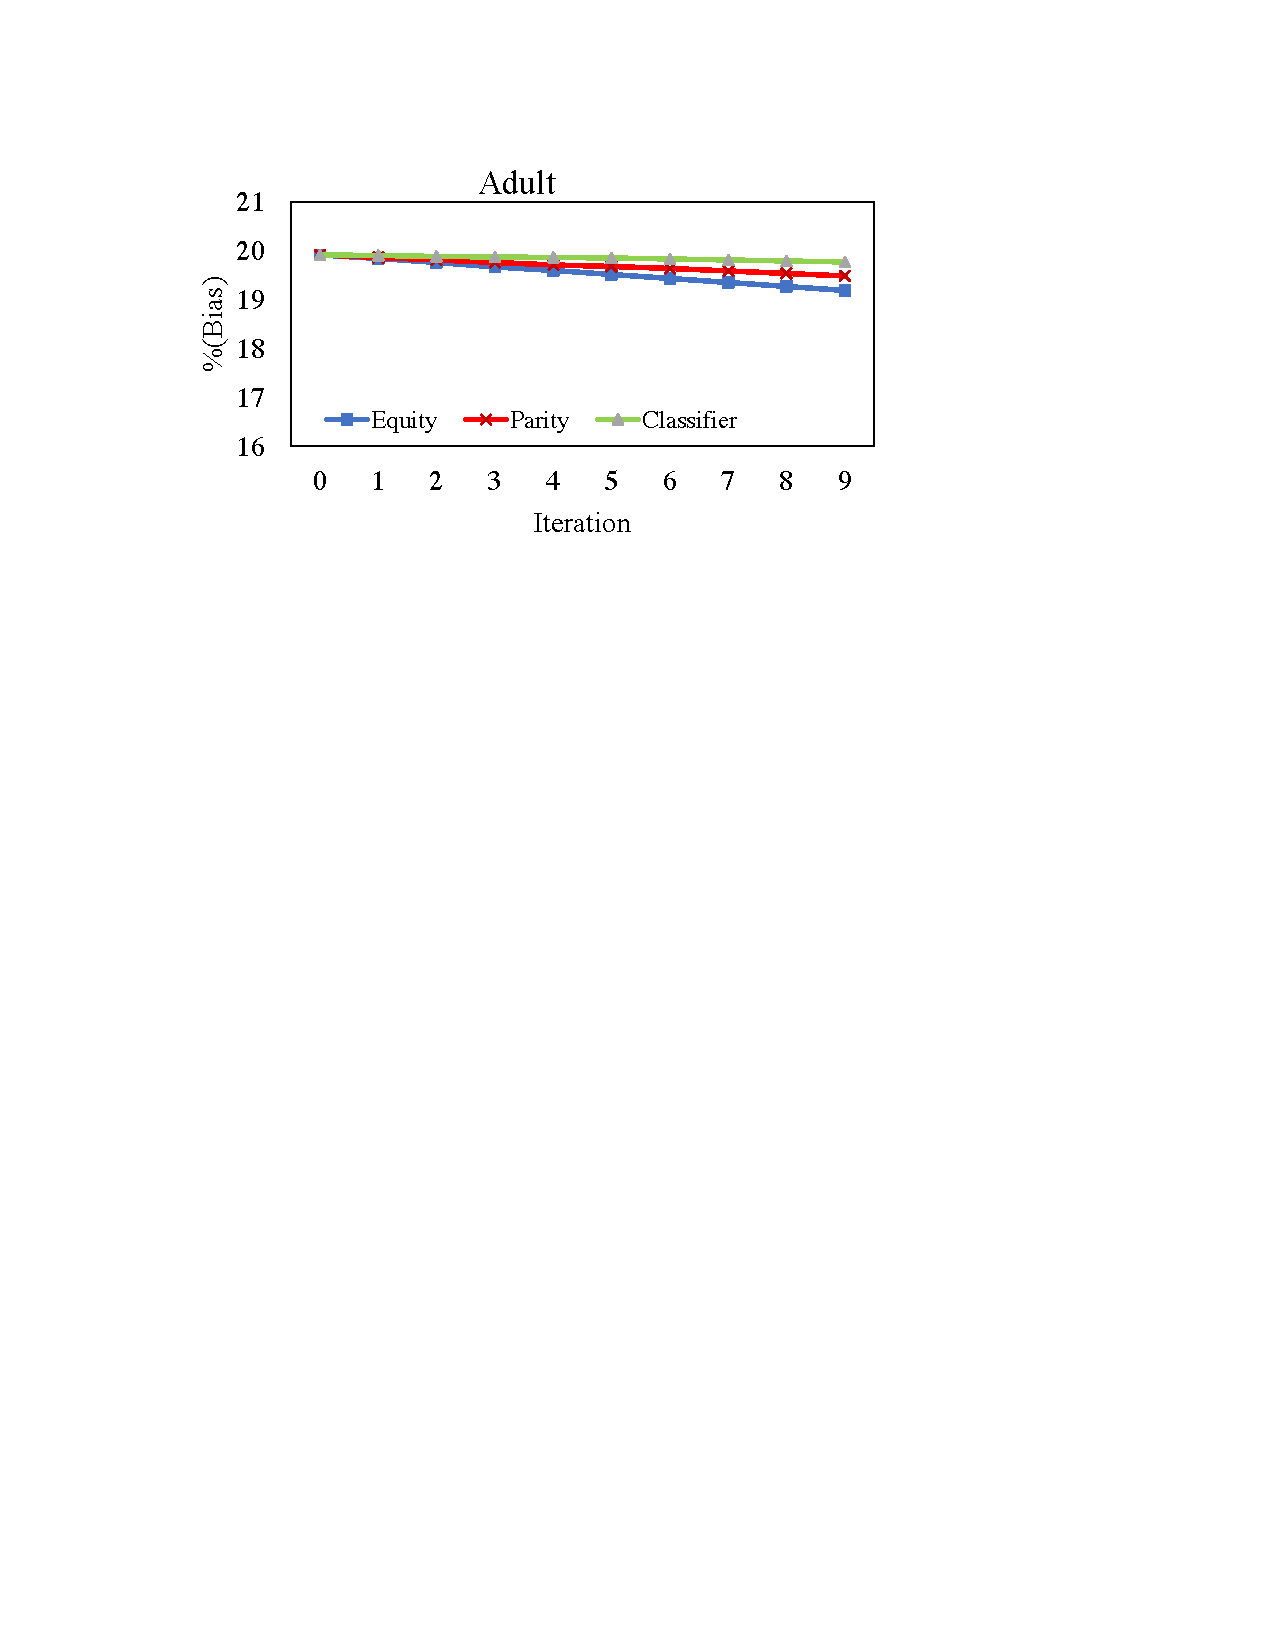
\includegraphics[width=\textwidth,trim=2.7cm 18cm 6.5cm 2.8cm,clip=true]{images/adult_per_01.pdf}
      \end{subfigure}
      \begin{subfigure}[b]{0.33\textwidth}
        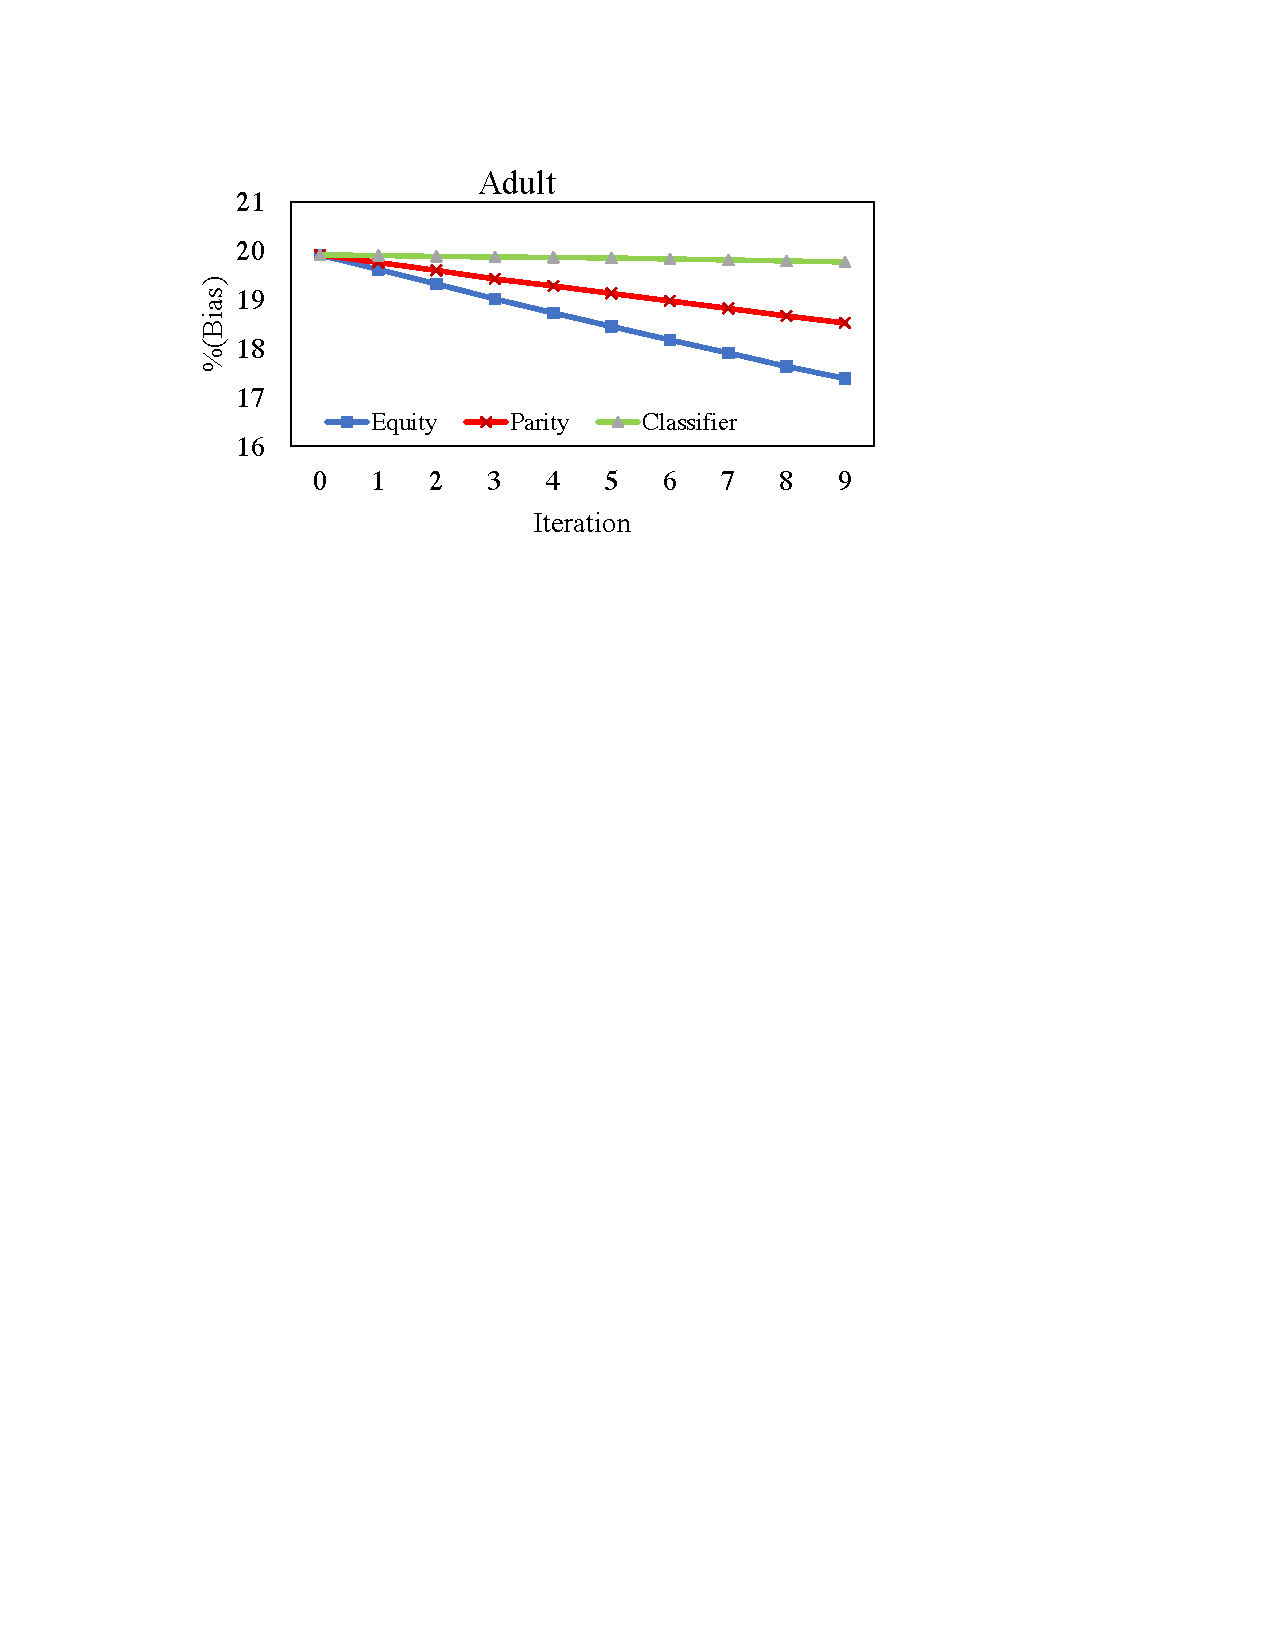
\includegraphics[width=\textwidth,trim=2.7cm 18cm 6.5cm 2.8cm,clip=true]{images/adult_per_05.pdf}
         \end{subfigure}
        \begin{subfigure}[b]{0.33\textwidth}
         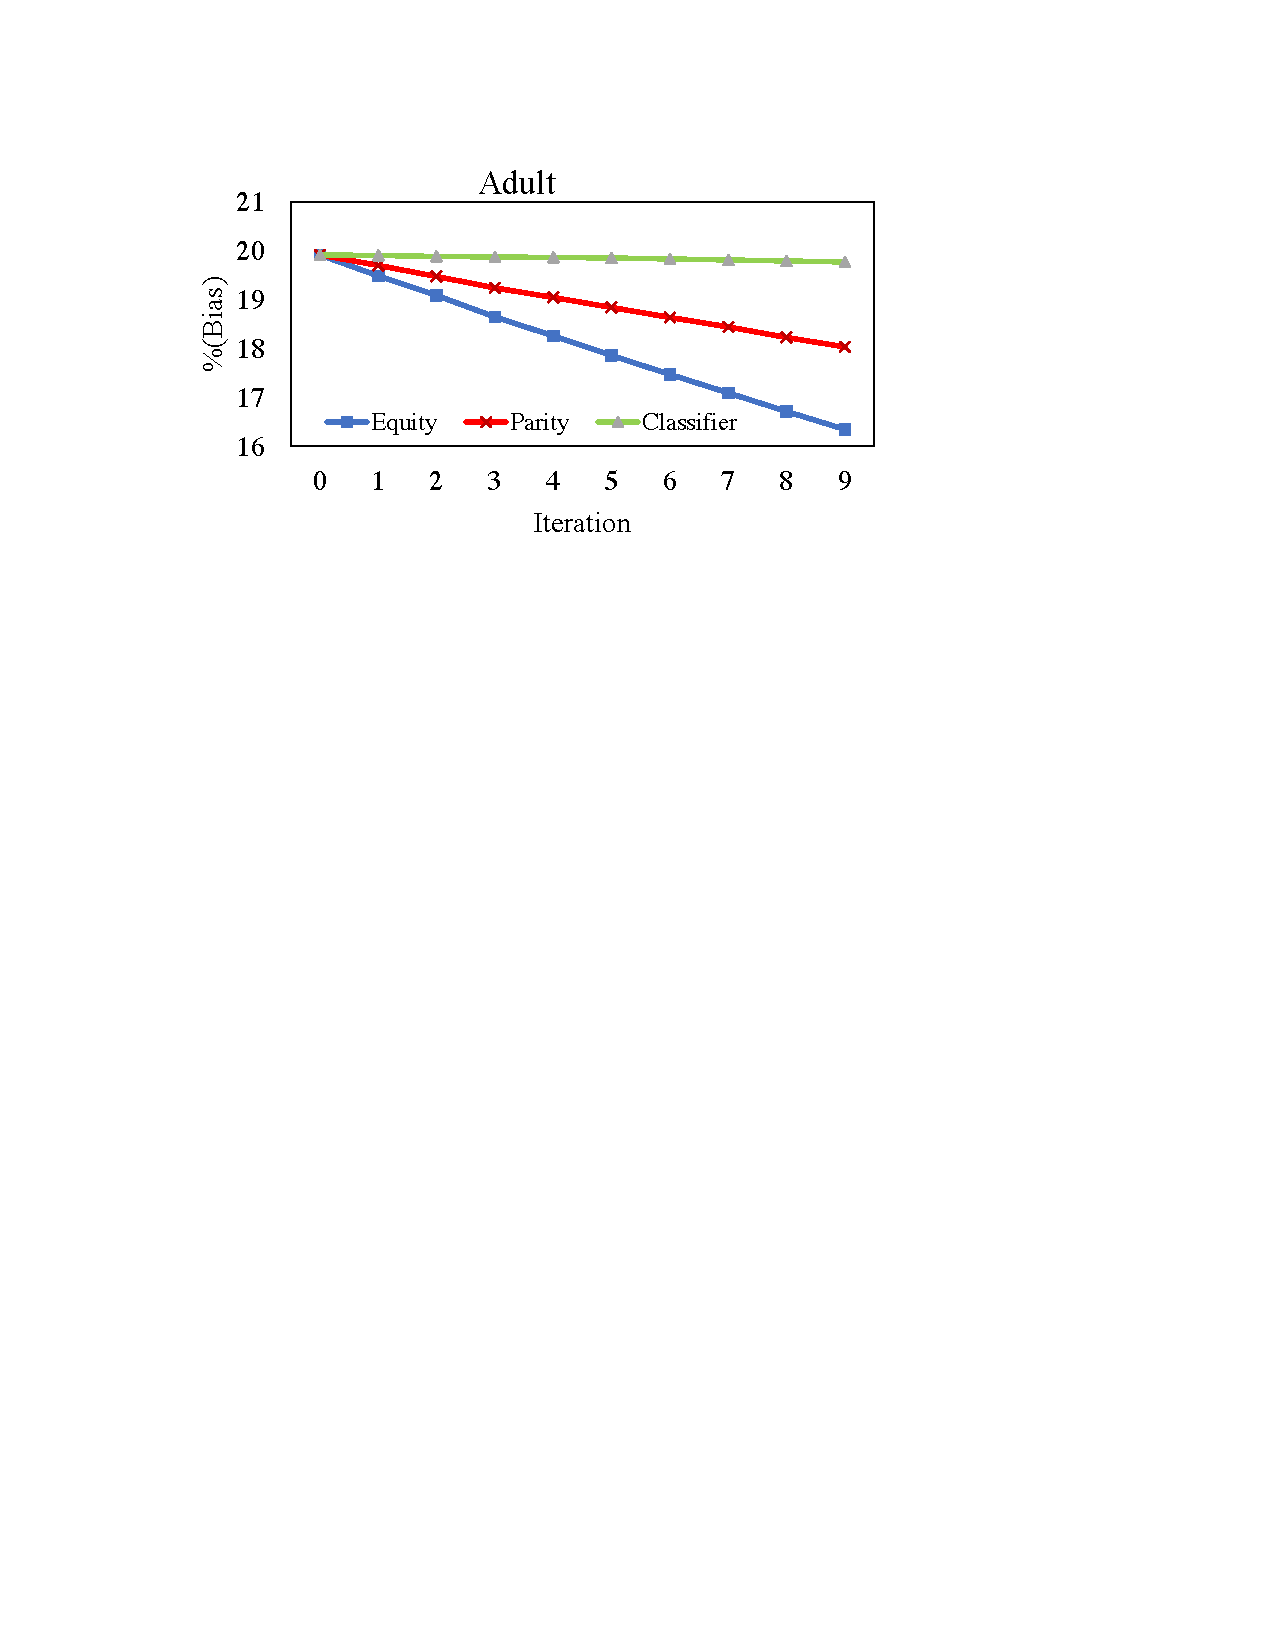
\includegraphics[width=\textwidth,trim=2.7cm 18cm 6.5cm 2.8cm,clip=true]{images/adult_per_09.pdf}
          \end{subfigure}
    \caption{Simulation of the feedback loop phenomenon and results obtained in reduction of bias via different methods in COMPAS and Adult datasets. As expected higher $\beta$ values result in reduction of more bias in the two fairness based objectives (Equity and Parity). It also shows how Equity is more effective in reducing the bias over iterations. Each point on the plots is the average value of 10 experiments performed on the 10 random splits. Notice that the 10 random split sets are the same across different $\beta$ values.}  
    \label{iteration_exp}
\end{figure*}
An important and major concern in the fairness community is the feedback loop phenomenon \cite{chouldechova2018frontiers}. Since biased data is generated by humans, these biases are perpetuated after the models make biased decisions based on the historical biased data. The bias originates from humans, the models amplify these biases, and they loop back biased results back to the humans. This loop gets repeated and continues to carry the initial existing biases. This phenomenon is called the feedback loop phenomenon.

We hope that since our notion considers and compensates the historical biases in the training set, which might have come from humans in initial phases, and attempts to fix them by achieving an ultimate equilibrium considering the past and future decisions, it may help with the mitigation of the feedback loop phenomenon. %This is another motivating reason for why we should consider historical biases and not only focus on equalizing the outcomes as historical biases exist and demographics should not be considered to be similar in the first place as this is an unrealistic assumption that is taken in some already existing fairness definitions \cite{Dwork:2012:FTA:2090236.2090255}.

In order to observe the effect of our new equity notion on fixing the historical biases in the training sets and effectively fixing the feedback loop as a consequence, we conducted experiments on datasets used in the previous section and recorded averaged results over the 10 experiments on random splits along with their Mann–Whitney U significance tests in this section with the following hypothesis. The model architecture remains the same as experiments conducted in the previous section. In addition the experiments are performed on the Equity, Parity, and Classification losses for comparison purposes.
\begin{tcolorbox}
\begin{hyp} 
The Equity classification objective can be the most effective in terms of reducing the disparities (bias) defined as $|p(Y|A=\text{a})-p(Y|A=\text{b})|$ between demographic groups $a$ and $b$ over some iterations when predictive outcomes on the test sets are accumulated over time on the historical train sets.
\end{hyp}
\end{tcolorbox}
\subsection{Experimental Design and Results}
Herein, we answer the question of what will happen if the equity classifier is allowed to play out in a realistic environment. We simulate the feedback loop as an iterative training-predicting cycle. We train our model in sequential chunks, splitting the test data into 10 equal-sized chunks. At the first iteration, we train the model using the train data. 
At each subsequent iteration, we take one of the chunks from our test data adding it to the previous train data alongside its \emph{predicted} labels and re-train the model for the next iteration. We then deleted this chunk from the test set and keep it in the train set. Each experiment was repeated 10 times with different random splits. 
\begin{table}[t]
\begin{tabular}{|p{0.5cm} |c||p{1.07cm}|p{1.15cm}||p{1.07cm}|p{1.15cm}|  }
 \hline
 \multicolumn{2}{|c||}{}&\multicolumn{2}{c||}{COMPAS Dataset}&\multicolumn{2}{c|}{Adult Dataset}\\
 \hline
 \multicolumn{2}{|c||}{}&\multicolumn{2}{c||}{$p$-value}&\multicolumn{2}{c|}{$p$-value}\\
 \hline
Iter& & Parity &Classifier&Parity&Classifier\\
 \hline
1&\multirow{8}{*}{\rotatebox[origin=c]{90}{Equity}}   & 0.1365    & 0.0809 & 0.0520& 0.0018\\
 2&    & 0.0520 &0.0106 &0.0045 &9.1e-05 \\
3&&0.0156 & 0.0004 &0.0002&9.1e-05\\
4&& 0.0070&  0.0002&9.1e-05&9.1e-05\\
5&& 0.0018& 0.0001 &9.1e-05&9.1e-05\\
6& &0.0006 & 9.1e-05 &9.1e-05&9.1e-05\\
7& &0.0008 & 9.1e-05 &9.1e-05&9.1e-05\\
8&&0.0004 &  9.1e-05&9.1e-05&9.1e-05\\
9&&0.0002 & 9.1e-05 &9.1e-05&9.1e-05\\
 \hline
\end{tabular}
\caption{Performance of Mann-Whitney U test for showing the effectiveness of Equity in reducing bias in the feedback loop compared to Parity and Classifier losses over different iterations for COMPAS and Adult datasets. The obtained $p$-values show the significance of our reported results in Figure \ref{iteration_exp} for $\beta$ value of 0.5.}
\label{05_feedbackloop_p}
\end{table}

Figure \ref{iteration_exp} reports $|p(Y|A=\text{female})-p(Y|A=\text{male})|$, averaged across 10 runs, as a measure for disparity for both predicted class labels $Y=0$ and $Y=1$ in each of the datasets for each of the fairness notions for each $\beta$ value. These results demonstrate that our notion of fairness was able to minimize the gap between $p(Y|A=\text{female})$ and $p(Y|A=\text{male})$ in all of the datasets. The results show that using our notion can bring equality, equity, and fairness in long run and mitigate the negative effects of the feedback loop phenomenon. As expected and shown in Figure \ref{iteration_exp}, higher $\beta$ values resulted in achieving more fair outcomes which resulted in reduction of bias. In addition, we reported the Mann–Whitney U test results to show the significance of our results. Table \ref{05_feedbackloop_p} shows the significance of these results for COMPAS and Adult datasets for $\beta$ value of 0.5 for different iterations supporting our hypothesis.\footnote{Results for other $\beta$ values  can be found in the \\ supplementary material.} This is consistent with our earlier finding that $\beta = 0.5$ is the most effective and reasonable with significant impact in gaining fairness, reducing bias, and balancing the fairness-accuracy trade-off. 

% \begin{figure}[h]
% \centering
%     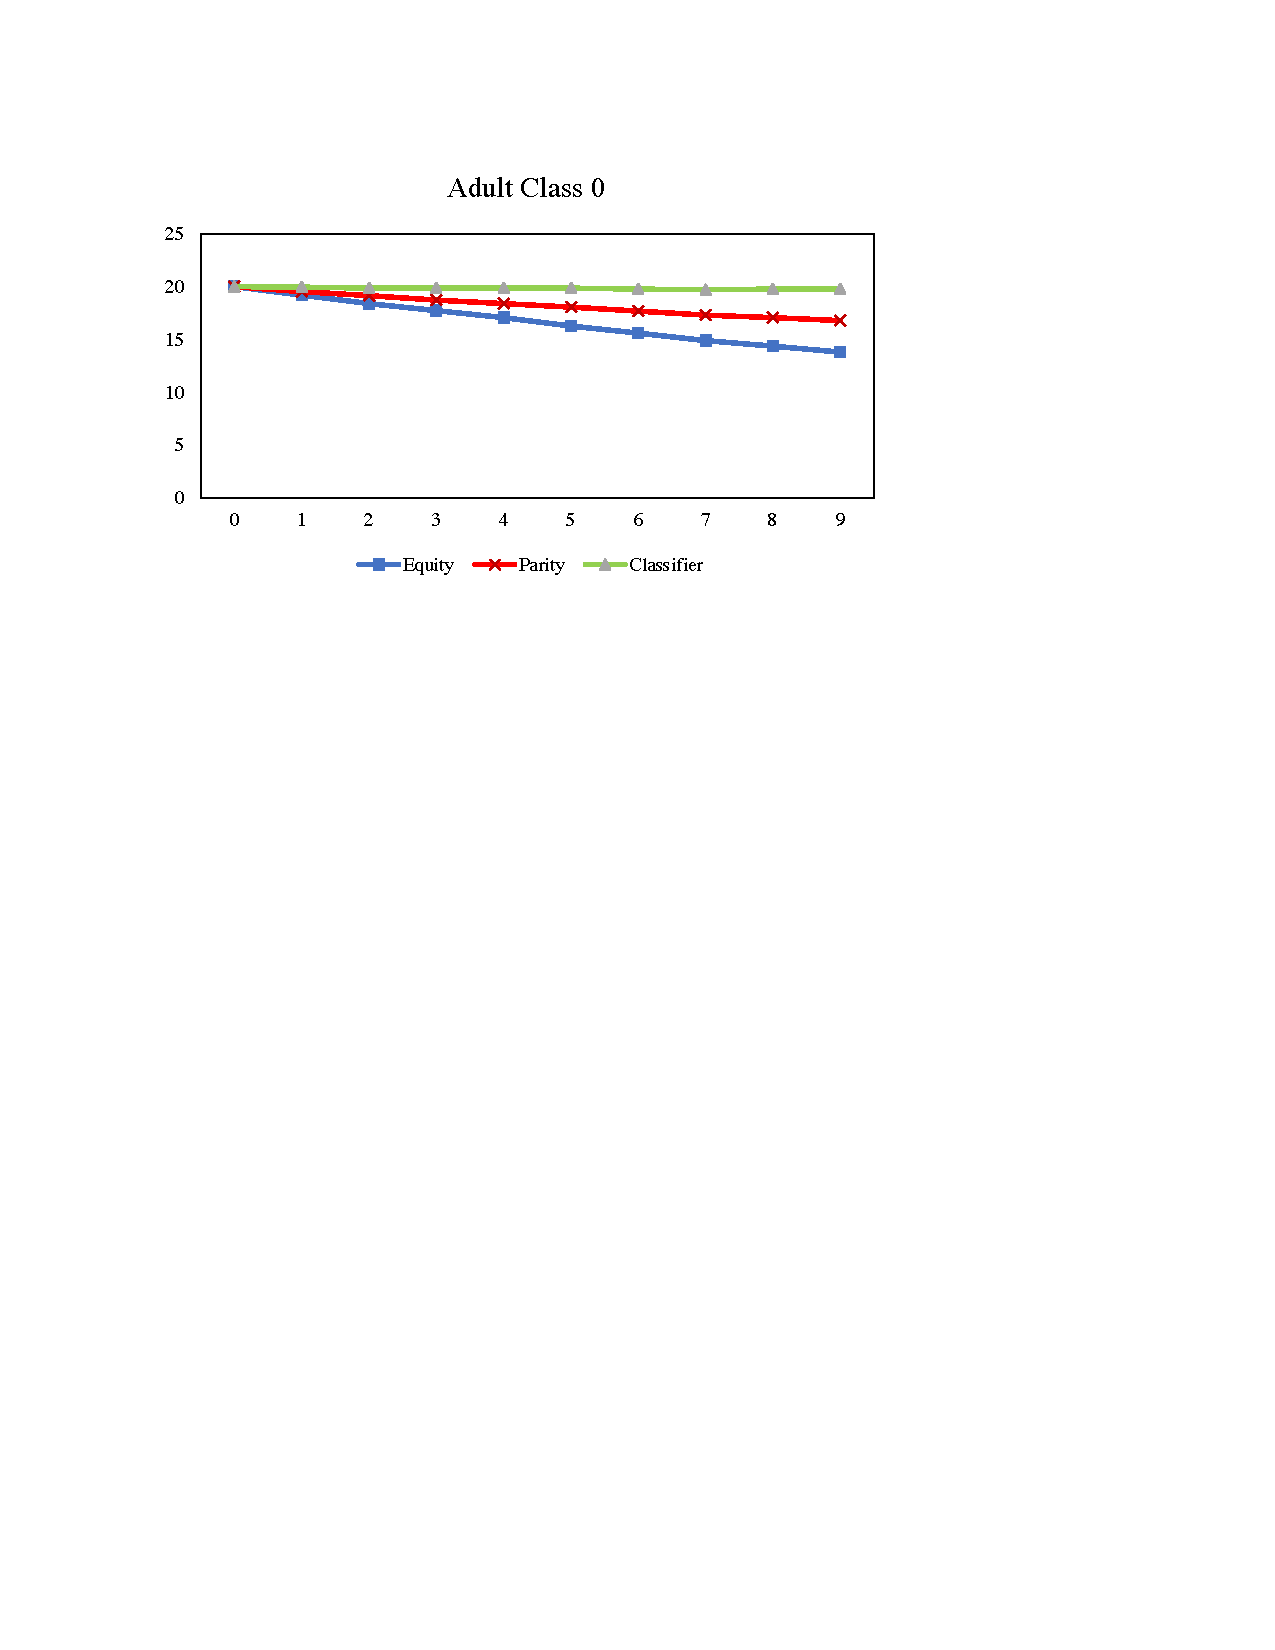
\includegraphics[width=0.22\textwidth,height=0.17\textwidth,trim=2.7cm 18cm 6cm 3cm,clip=true]{images/adult_iter_0.pdf}
%      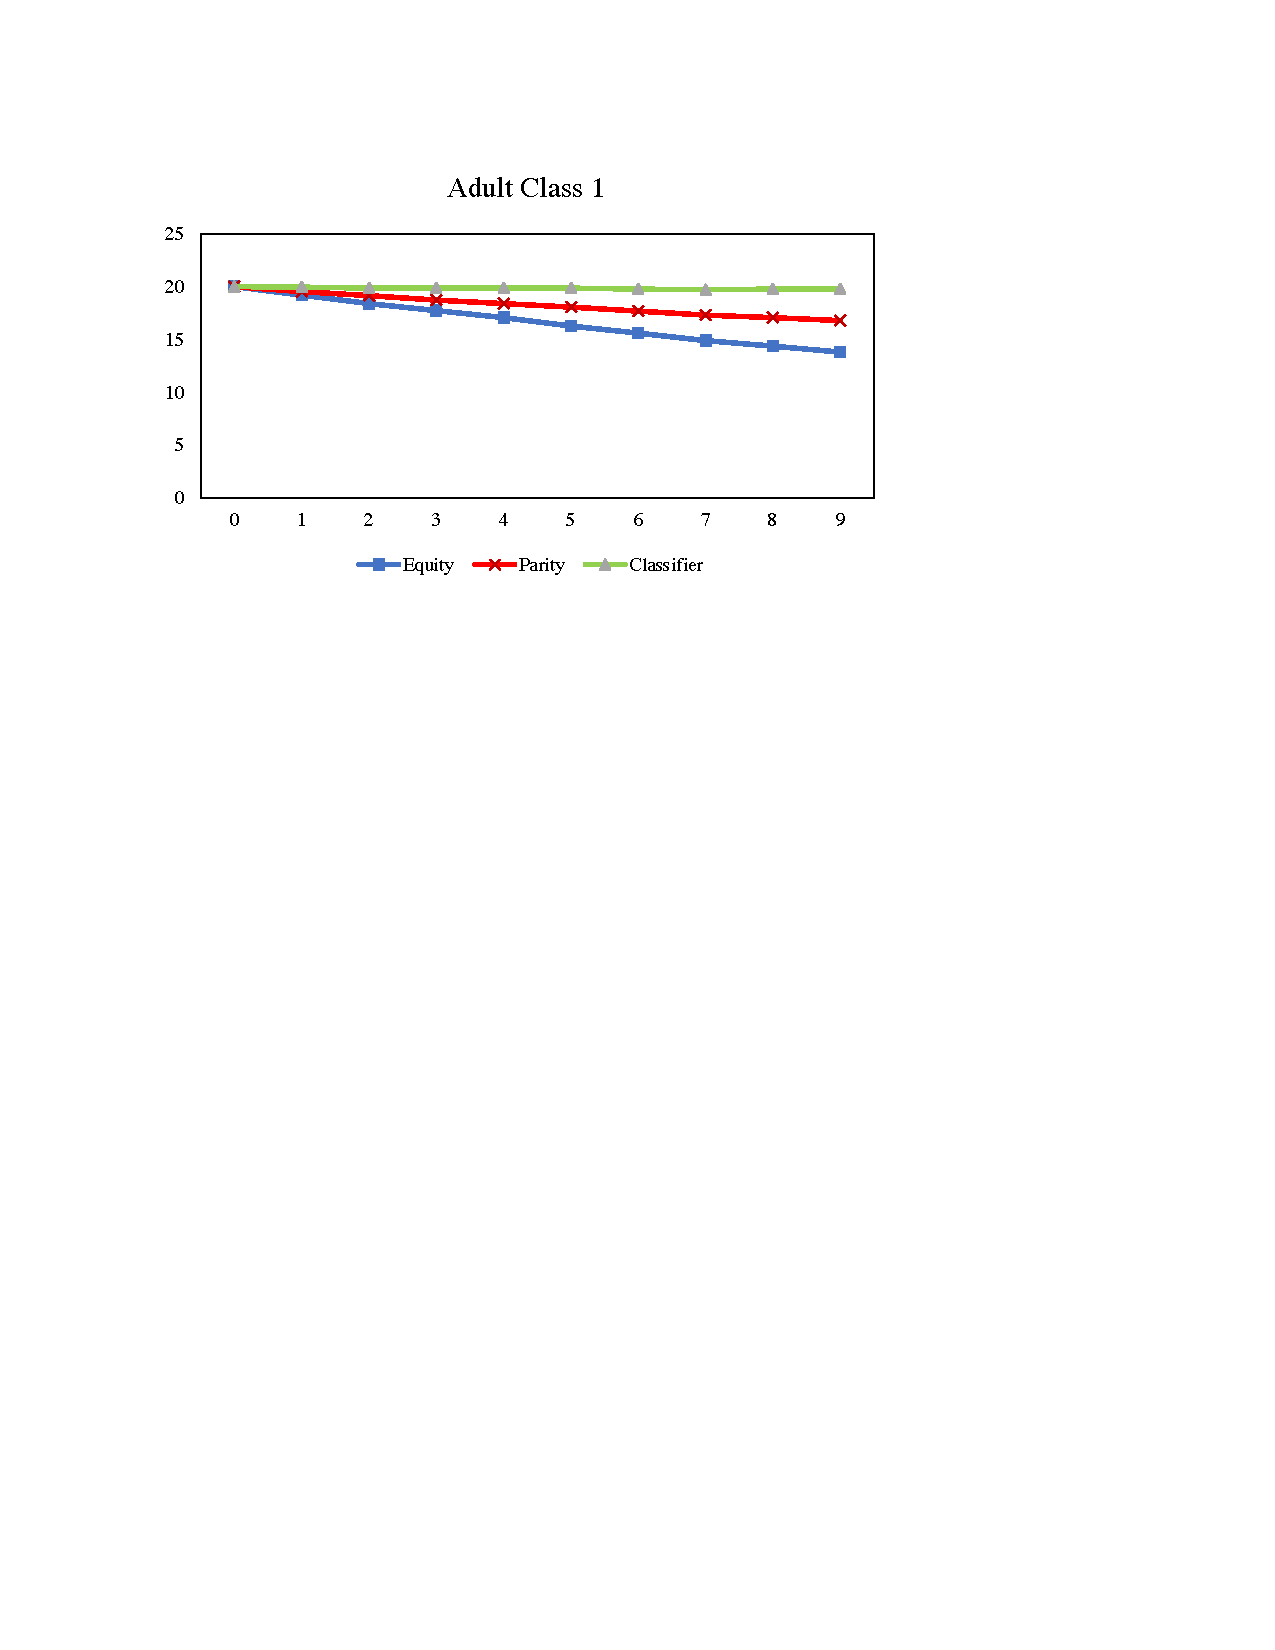
\includegraphics[width=0.22\textwidth,height=0.17\textwidth,trim=2.7cm 18cm 6cm 3cm,clip=true]{images/adult_iter_1.pdf}
%       \includegraphics[width=0.22\textwidth,height=0.17\textwidth,trim=2.7cm 18cm 6cm 3cm,clip=true]{images/german_iter_0.pdf}
%       \includegraphics[width=0.22\textwidth,height=0.17\textwidth,trim=2.7cm 18cm 6cm 3cm,clip=true]{images/german_iter_1.pdf}
%         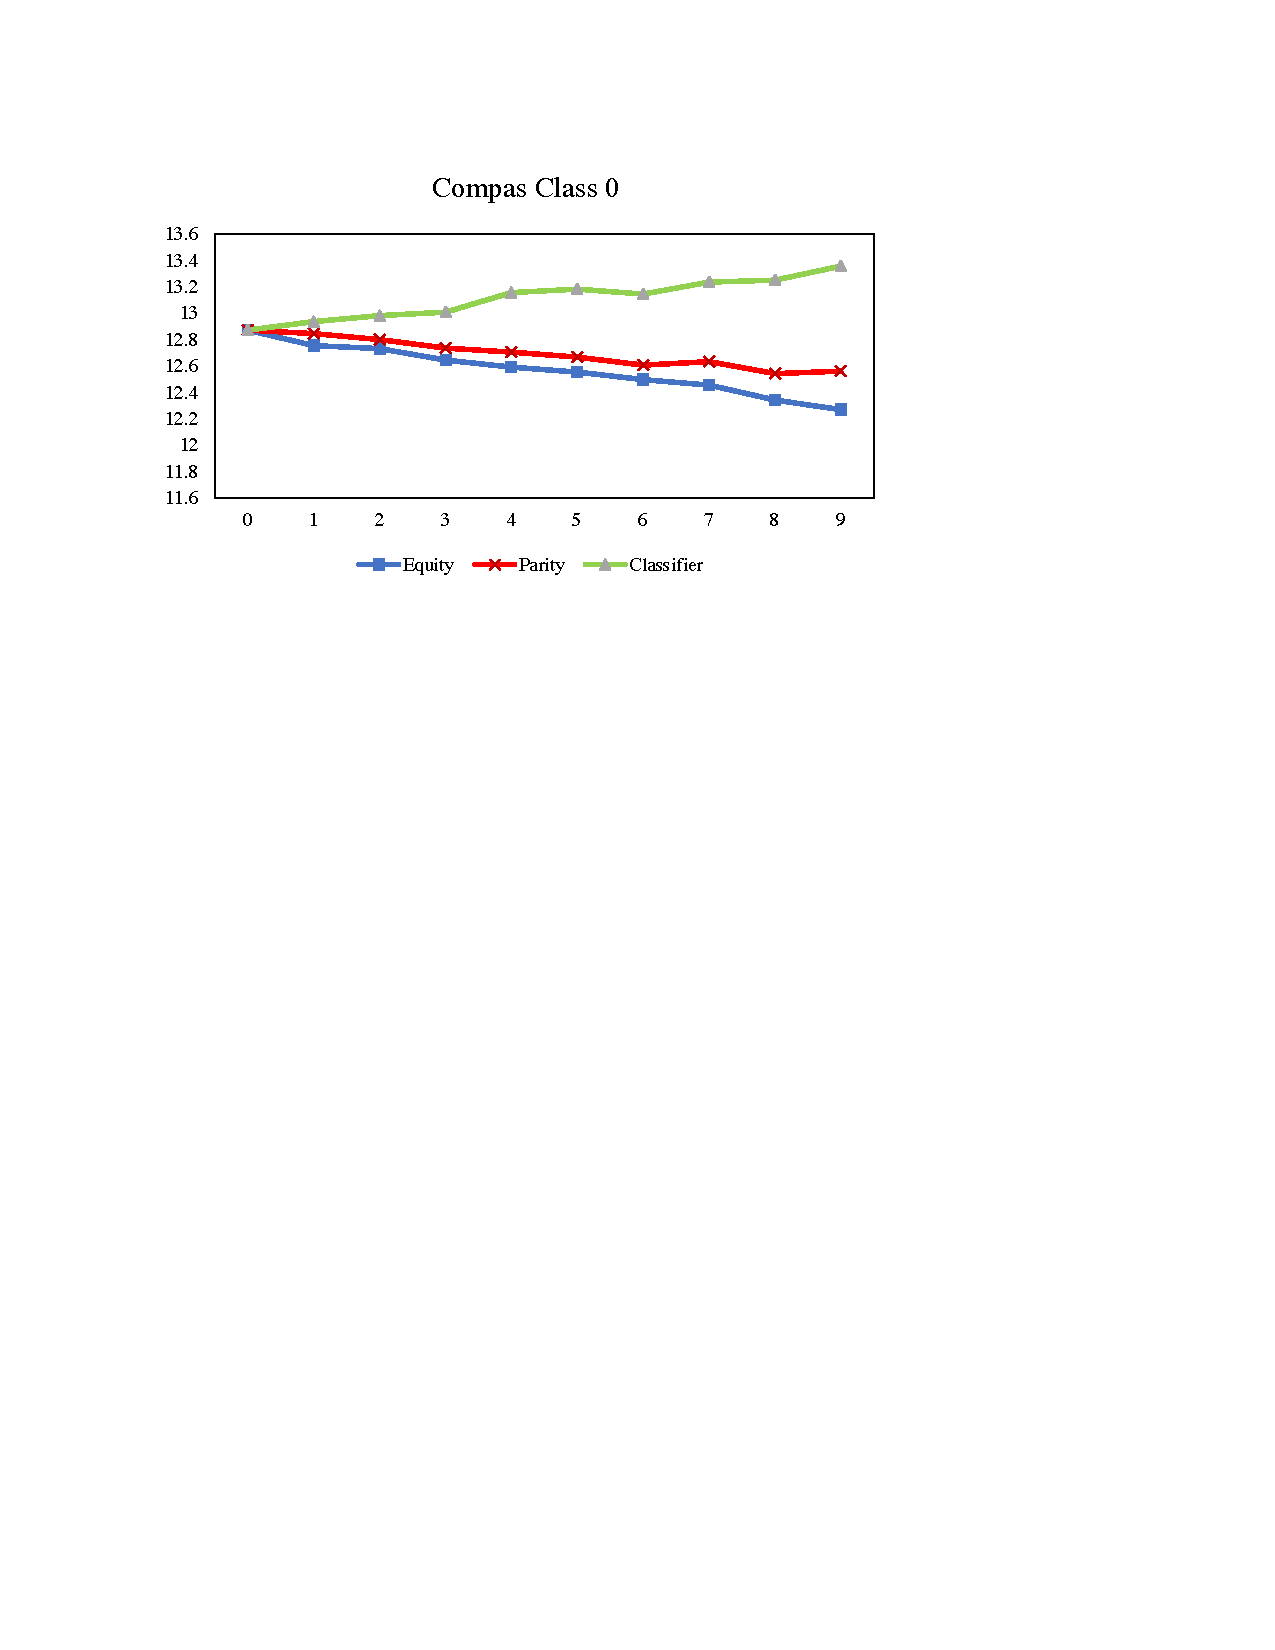
\includegraphics[width=0.22\textwidth,height=0.17\textwidth,trim=2.7cm 18cm 6cm 3cm,clip=true]{images/compas_iter_0.pdf}
%          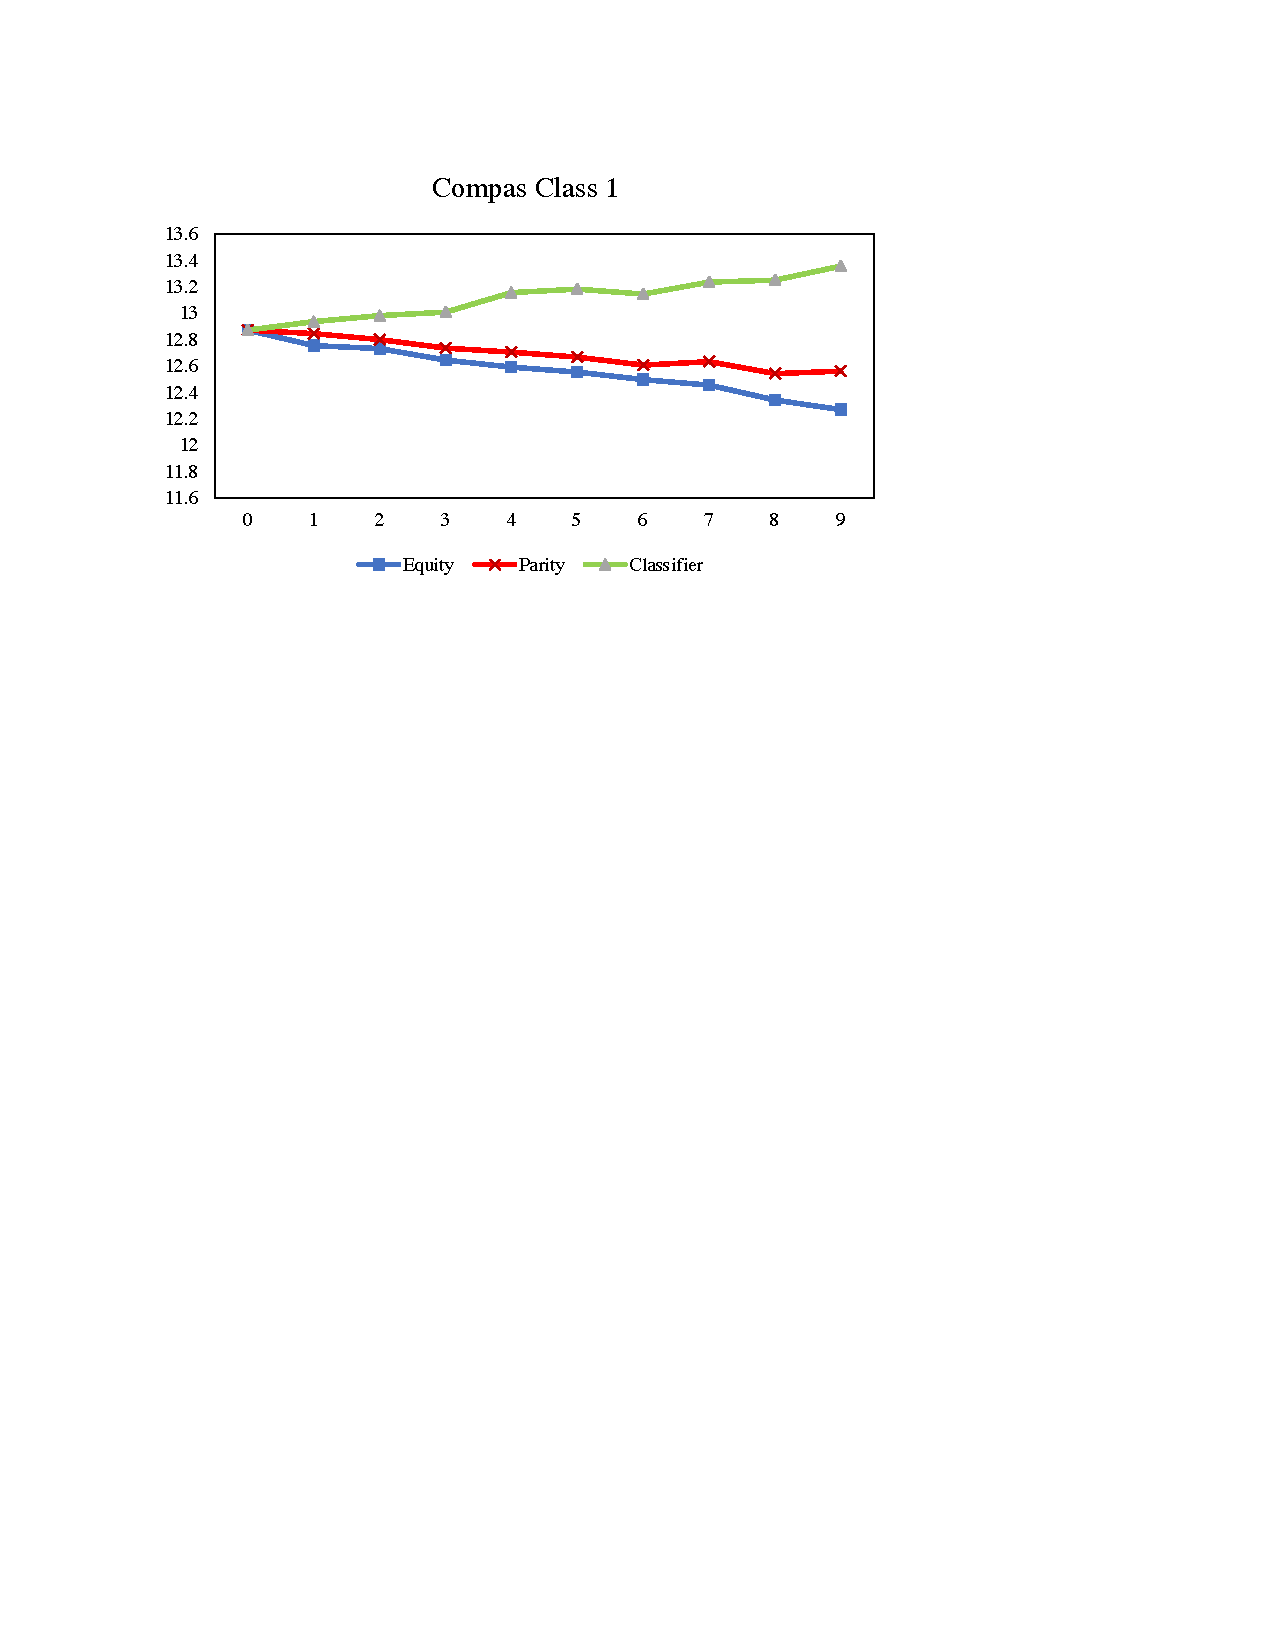
\includegraphics[width=0.22\textwidth,height=0.17\textwidth,trim=2.7cm 18cm 6cm 3cm,clip=true]{images/compas_iter_1.pdf}
%     \caption{}
%     \label{iteration_exp}
% \end{figure}


% \begin{figure*}[h]
% \centering
% \begin{subfigure}[b]{0.33\textwidth}
% \caption{$\beta=0.1$}
%     \includegraphics[width=\textwidth,height=0.5\textwidth,trim=2.7cm 18cm 6.5cm 2.8cm,clip=true]{images/final_compas_01.pdf}
%     \end{subfigure}
%     \begin{subfigure}[b]{0.33\textwidth}
% \caption{$\beta=0.5$}
%      \includegraphics[width=\textwidth,height=0.5\textwidth,trim=2.7cm 18cm 6.5cm 2.8cm,clip=true]{images/final_compas_05.pdf}
%       \end{subfigure}
%      \begin{subfigure}[b]{0.33\textwidth}
% \caption{$\beta=0.9$}
%       \includegraphics[width=\textwidth,height=0.5\textwidth,trim=2.7cm 18cm 6.5cm 2.8cm,clip=true]{images/final_compas_09.pdf}
%       \end{subfigure}
%       \begin{subfigure}[b]{0.33\textwidth}
%       \includegraphics[width=\textwidth,height=0.5\textwidth,trim=2.7cm 18cm 6.5cm 2.8cm,clip=true]{images/final_adult_01.pdf}
%       \end{subfigure}
%       \begin{subfigure}[b]{0.33\textwidth}
%         \includegraphics[width=\textwidth,height=0.5\textwidth,trim=2.7cm 18cm 6.5cm 2.8cm,clip=true]{images/final_adult_05.pdf}
%          \end{subfigure}
%         \begin{subfigure}[b]{0.33\textwidth}
%          \includegraphics[width=\textwidth,height=0.5\textwidth,trim=2.7cm 18cm 6.5cm 2.8cm,clip=true]{images/final_adult_09.pdf}
%           \end{subfigure}
%          \begin{subfigure}[b]{0.33\textwidth}
%           \includegraphics[width=\textwidth,height=0.5\textwidth,trim=2.7cm 18cm 6.5cm 2.8cm,clip=true]{images/final_german_01.pdf}
%           \end{subfigure}
%           \begin{subfigure}[b]{0.33\textwidth}
%      \includegraphics[width=\textwidth,height=0.5\textwidth,trim=2.7cm 18cm 6.5cm 2.8cm,clip=true]{images/final_german_05.pdf}
%       \end{subfigure}
%      \begin{subfigure}[b]{0.33\textwidth}
%      \includegraphics[width=\textwidth,height=0.5\textwidth,trim=2.7cm 18cm 6.5cm 2.8cm,clip=true]{images/final_german_09.pdf}
%       \end{subfigure}
%     \caption{}
%     \label{iteration_exp}
% \end{figure*}


